\chapter{Seznam již vydaných videí} \label{released-videos}
Tato příloha obsahuje kompletní seznam videí vzniklých v~rámci projektu P3D vč. odkazů rozdělených dle jednotlivých témat. \newline
\noindent\It{Pozn.: při kliknutí na odkaz budete přesměrování na stránku korespondujícího videa (pouze v~digitální verzi)}.

\section{Instalace a zprovoznění SolidWorks SDK} \label{videa-instalace}
\href{https://aka.parallaxproduction.cz/instalaceSDK}{Instalace a první spuštění SolidWorks SDK 2020/2021 (aka.parallaxproduction.cz/instSDK)} \newline
\href{https://aka.parallaxproduction.cz/sablony}{Instalace šablon a knihoven norm. dílů ze Sokolské (aka.parallaxproduction.cz/sablony)} \newline
\href{https://aka.parallaxproduction.cz/realview}{Aktivace Realview na necertifikované grafické kartě (aka.parallaxproduction.cz/realview)} \newline

\section{Základy modelování} \label{videa-modelovani}
\href{https://aka.parallaxproduction.cz/jednoducha-pruzina}{Jednoduchá pružina (aka.parallaxproduction.cz/jednoducha-pruzina)} \newline
\href{https://aka.parallaxproduction.cz/j-ozubene-kolo}{Ozubené kolo s~přímým čelním ozubením (aka.parallaxproduction.cz/j-ozubene-kolo)} \newline
\href{https://aka.parallaxproduction.cz/vyk-oz-kolo}{Ozubené kolo pro výkres - obálka (aka.parallaxproduction.cz/vyk-oz-kolo)} \newline
\href{https://aka.parallaxproduction.cz/jednorad-r-kolo}{Jednořadé řetězové kolo (aka.parallaxproduction.cz/jednorad-r-kolo)} \newline
\href{https://aka.parallaxproduction.cz/perodrazka-naboj}{Drážka pro pero v~náboji (aka.parallaxproduction.cz/perodrazka-naboj)} \newline
\href{https://aka.parallaxproduction.cz/perodrazka-hridel}{Drážka pro pero na hřídeli (aka.parallaxproduction.cz/perodrazka-hridel)} \newline

\section{Výkresová dokumentace} \label{videa-vykresy}
\href{https://aka.parallaxproduction.cz/popisove-pole}{Popisové pole a už. vlastnosti na výkrese (aka.parallaxproduction.cz/popisove-pole)} \newline
\href{https://aka.parallaxproduction.cz/vykres-perodrazka-na}{Výkres drážky pro pero v~náboji (aka.parallaxproduction.cz/vykres-perodrazka-hr)} \newline
\href{https://aka.parallaxproduction.cz/vykres-perodrazka-hr}{Výkres drážky pro pero na hřídeli (aka.parallaxproduction.cz/vykres-perodrazka-hr)} \newline

\section{Práce se sestavami} \label{videa-sestavy}
\href{https://aka.parallaxproduction.cz/prejmenovani-dilu}{Přejmenování dílu v~sestavě (aka.parallaxproduction.cz/prejmenovani-dilu)} \newline
\href{https://aka.parallaxproduction.cz/pack-and-go}{Přesun sestavy pomocí Pack and Go... (aka.parallaxproduction.cz/pack-and-go)} \newline

\chapter{Seznam plánovaných témat} \label{planned-videos}
V~následujícím seznamu naleznete další témata, pro která jsou videa plánována.

\subsection*{Nastavení a úpravy SolidWorks}
\begin{itemize}
    \setlength\itemsep{0.05em}
    \item Upgrade SolidWorks na novou verzi (např. 2020 na 2021),
    \item vlastní úpravy uživatelského prostředí,
    \item doplňkové moduly SolidWorks.
\end{itemize}

\subsection*{Základy modelování}
\begin{itemize}
    \setlength\itemsep{0.05em}
    \item Řetěz,
    \item řemen,
    \item plechové díly (série),
    \item svařované konstrukce (série),
    \item další normalizované prvky.
\end{itemize}

\subsection*{Výkresová dokumentace}
\begin{itemize}
    \setlength\itemsep{0.05em}
    \item Kusovník na výkrese sestavy,
    \item 
\end{itemize}

\subsection*{Sestavy}
\begin{itemize}
    \setlength\itemsep{0.05em}
    \item Základní, upřesňující a strojní vazby (série),
    \item konfigurace (pravděpodobně série).
\end{itemize}

%\chapter{Obrazové přílohy}

%\begin{figure}[h]
%    \centering
%    \includegraphics[width=0.85\textwidth]{img/ToBeRemoved/PPSB-T_BOTH.png}
%    \caption{Vizualizace PPSB-T (horní strana vpravo, dolní vlevo).}
%    \label{fig:PPSB-T_VISUAL}
%\end{figure}

\chapter{Vybrané normy}

\begin{table}[] \catcode`\-=12
    \centering
    \begin{tabular}{c|cc|c|c|c|ccccc}
    \multirow{2}{*}{\B{Průměr D}} & \multicolumn{3}{c|}{\B{Rozměr drážky}}      & \multicolumn{2}{c|}{\B{Mezní úchylky hloubky}}                                                                                              & \multicolumn{5}{c}{\B{Rozměry pera}}                                  \\ \cline{2-11} 
                                  & t   & t\subscript{1} & R\subscript{1}       & \multicolumn{1}{l|}{na hřídeli (t)}                                  & \multicolumn{1}{l|}{v náboji (t\subscript{1})}                       & b  & h  & R                     & l\subscript{min} & l\subscript{max} \\ \hline
    6 až 8                        & 1,1 & 0,9            & \multirow{2}{*}{0,2} & \multirow{4}{*}{\begin{tabular}[c]{@{}c@{}}+0,1\\ -0,0\end{tabular}} & \multirow{9}{*}{\begin{tabular}[c]{@{}c@{}}+0,2\\ +0,1\end{tabular}} & 2  & 2  & \multirow{2}{*}{0,25} & 9                & 20               \\
    8 až 10                       & 1,7 & 1,3            &                      &                                                                      &                                                                      & 3  & 3  &                       & 9                & 36               \\ \cline{1-4} \cline{7-11} 
    10 až 12                      & 2,4 & 1,6            & \multirow{4}{*}{0,4} &                                                                      &                                                                      & 4  & 4  & \multirow{4}{*}{0,5}  & 10               & 45               \\
    12 až 17                      & 2,9 & 2,1            &                      &                                                                      &                                                                      & 5  & 5  &                       & 12               & 56               \\ \cline{5-5}
    17 až 22                      & 3,5 & 2,5            &                      & \multirow{8}{*}{\begin{tabular}[c]{@{}c@{}}+0,2\\ -0,0\end{tabular}} &                                                                      & 6  & 6  &                       & 16               & 70               \\
    22 až 30                      & 4,1 & 2,9            &                      &                                                                      &                                                                      & 8  & 7  &                       & 20               & 90               \\ \cline{1-4} \cline{7-11} 
    30 až 38                      & 4,7 & 3,3            & \multirow{6}{*}{0,6} &                                                                      &                                                                      & 10 & 8  & \multirow{6}{*}{0,7}  & 25               & 110              \\
    38 až 44                      & 4,9 & 3,1            &                      &                                                                      &                                                                      & 12 & 8  &                       & 32               & 140              \\
    44 až 50                      & 5,5 & 3,5            &                      &                                                                      &                                                                      & 14 & 9  &                       & 40               & 180              \\ \cline{6-6}
    50 až 58                      & 6,2 & 3,8            &                      &                                                                      & \multirow{3}{*}{\begin{tabular}[c]{@{}c@{}}+0,4\\ +0,2\end{tabular}} & 16 & 10 &                       & 45               & 200              \\
    58 až 65                      & 6,8 & 4,2            &                      &                                                                      &                                                                      & 18 & 11 &                       & 50               & 220              \\
    65 až 75                      & 7,4 & 4,6            &                      &                                                                      &                                                                      & 20 & 12 &                       & 56               & 250             
    \end{tabular}
    \caption{Výběr z~normy ČSN 02 2562 - Pera těsná\cite{ST}}
    \label{tab:pera-tesna}
\end{table}

\begin{figure}[htbp]
    \centering
    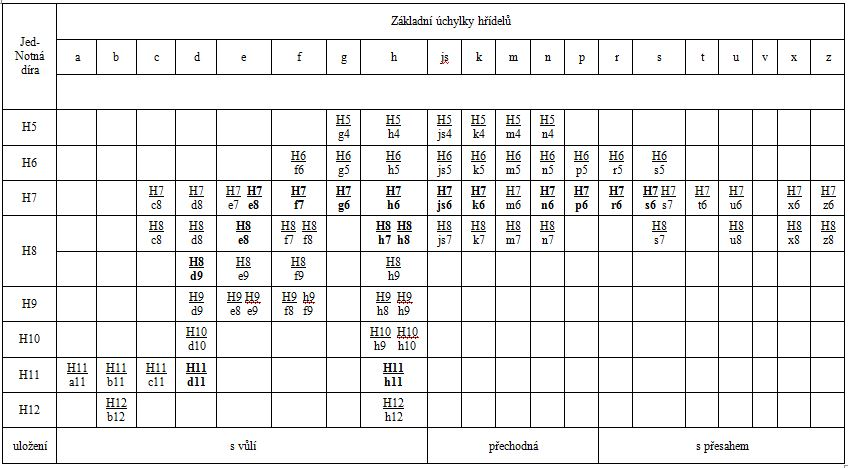
\includegraphics[width=1\textwidth]{img/jednotna-dira.JPG}
    \caption{Soustava jednotné díry, tučně zvýrazněné hodnoty jsou doporučené, převzato z~\cite{ELUC-DIRA}}
    \label{fig:jednotna-dira}
\end{figure}

\begin{figure}[htbp]
    \centering
    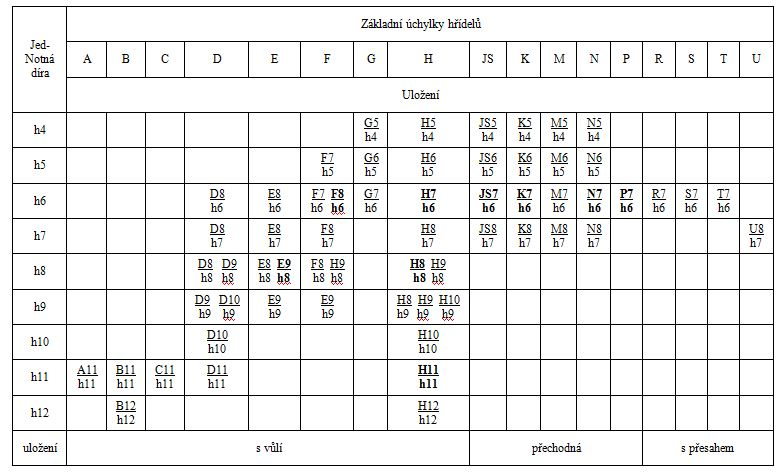
\includegraphics[width=1\textwidth]{img/jednotna-hridel.JPG}
    \caption{Soustava jednotného hřídele, tučně zvýrazněné hodnoty jsou doporučené, převzato z~\cite{ELUC-HRIDEL}}
    \label{fig:jednotna-hridel}
\end{figure}